\documentclass[12pt, a4paper, oneside]{Thesis} % Paper size, default font size and one-sided paper
\usepackage{wrapfig}
\usepackage{lscape}
\usepackage{rotating}
\usepackage{graphicx}
\usepackage{caption}
\usepackage{amsmath}
\usepackage[boxed]{algorithm}
\usepackage[noend]{algpseudocode}



\usepackage{lineno,hyperref}
\modulolinenumbers[5]


\usepackage{amssymb}
\usepackage{graphicx}
\usepackage{array}
\usepackage{float}
\usepackage{placeins}
\usepackage{stackengine}
\usepackage{url}
\usepackage{numprint}
\usepackage{caption}

\usepackage{booktabs}  
\usepackage{siunitx}
%\usepackage[showframe=false]{geometry}
\usepackage{subfigure}

\nprounddigits{3}
\newcolumntype{P}[1]{>{\centering\arraybackslash}p{#1}}
\newcolumntype{M}[1]{>{\centering\arraybackslash}m{#1}}

\setstackEOL{\#}
\setstackgap{L}{12pt}


%\usepackage{subcaption} %incompatible with subfig
\graphicspath{{Pictures/}} % Specifies the directory where pictures are stored
\usepackage[numbers,square]{natbib} % Use the natbib reference package - read up on this to edit the reference style; if you want text (e.g. Smith et al., 2012) for the in-text references (instead of numbers), remove 'numbers' v

\hypersetup{urlcolor=black, colorlinks=false} % Colors hyperlinks in blue - change to black if annoyingv`	

\thesistitle{Locality aware scheduling optimizations for CNN pipelines}
\supervisor{Professor Soumyajit Dey}
\degree{Dual Degree (B.Tech + M.Tech)}
\degreemajor{Electronics \& Electrical Communications Engineering}
\authors{Pankaj Mishra}
\rollno{17EC35034}
\university{Indian Institute of Technology Kharagpur}
\department{Department of Electronics \& Electrical Communications Engineering}
\unisite{http://www.iitkgp.ac.in}
\depsite{http://ece.iitkgp.ac.in/}
\placeshrt{Kharagpur}
\placelng{Kharagpur - 721302, India}
\datesub{November 20, 2020}
\datesig{November 20, 2020}
\semsub{Autumn Semester, 2020-21}
\keywords{High Performance Computing}
\coursecd{B.Tech Project - I Thesis }

\title{\ttitle} % Defines the thesis title - don't touch this
\begin{document}
%\makeatletter
%\renewcommand*{\NAT@nmfmt}[1]{\textsc{#1}}
%\makeatother

% prints author names as small caps


\frontmatter % Use roman page numbering style (i, ii, iii, iv...) for the pre-content pages

\setstretch{1.6} % Line spacing of 1.6 (double line spacing)

% Define the page headers using the FancyHdr package and set up for one-sided printing
\fancyhead{} % Clears all page headers and footers
\rhead{\thepage} % Sets the right side header to show the page number
\lhead{} % Clears the left side page header

%\pagestyle{fancy} % Finally, use the "fancy" page style to implement the FancyHdr headers

\newcommand{\HRule}{\rule{\linewidth}{0.5mm}} % New command to make the lines in the title page

% PDF meta-data
\hypersetup{pdftitle={\ttitle}}
\hypersetup{pdfsubject=\subjectname}
\hypersetup{pdfauthor=\authornames}
\hypersetup{pdfkeywords=\keywordnames}

%----------------------------------------------------------------------------------------
%	TITLE PAGE
%----------------------------------------------------------------------------------------
\maketitle
%\titlepg % Add a gap in the Contents, for aesthetics

\clearpage % Start a new page

%----------------------------------------------------------------------------------------
%	DECLARATION PAGE
%	Your institution may give you a different text to place here
%----------------------------------------------------------------------------------------


\Declaration% Add a gap in the Contents, for aesthetics


%----------------------------------------------------------------------------------------
%	CERTIFICATE PAGE
%----------------------------------------------------------------------------------------

% \addtotoc{Certificate} % Add the "Abstract" page entry to the Contents

% \certificate{\addtocontents{toc}{}} % Add a gap in the Contents, for aesthetics

\clearpage % Start a new page

%----------------------------------------------------------------------------------------
%	ABSTRACT PAGE
%----------------------------------------------------------------------------------------

\addtotoc{Abstract} % Add the "Abstract" page entry to the Contents

\abstract{\addtocontents{toc}{} % Add a gap in the Contents, for aesthetics
% The past decade has seen diminishing returns from Moore's Law because of increasing fabrication costs,
% technological barriers and power density limits. As a result Heterogeneous Computing architectures (like multi-core CPUs with a GPU) have been adopted almost universally to optimise performance. 
% These architectures have been complemented well by parallel programming languages like CUDA and OpenCL which have been used to build several high performance solutions in a diverse set of fields.
% The focus of this thesis is the latter i.e. OpenCL, due to it being the most pervasive, cross-vendor, open standard for heterogenous parallel programming. 
% Inspite of the ubiquitous nature of heterogenous computing, programmers require a considerable amount of expertise to efficiently design data parallel algorithms. Further, due to the low level nature of OpenCL, there is a lot of programming 
% overhead to ensure correctness during execution and data transfer via synchornisation. The primary aim of 
% our framework - PyschedCL is to address the above issues in designing OpenCL applications and help a novice
% end user bridge the gap between homogenous and heterogenous computing systems. It completely eliminates the programming overhead by automating 
% the synchornisation routines to ensure correctness. The scheduling backend also comprises of a Machine Learning based 
% scheduling policy which can intelligently map the underlying elements of an application to the target heterogenous platform. The modular nature of the framework allows the user to 
% replace the scheduling policy of the backend with a custom scheduling algorithm too. This can help researchers design and validate several scheduling algorithms. The framework tries to exploit 



Over the past years, there has been a steady growth in the performance capabilities of GPGPU platforms which have led to the popularity of parallel programming models such as CUDA by Nvidia. However, despite the massive increase in the compute ability of these platforms thanks to an exponential rise in the hardware-level parallelism they offer, software-level optimizations still fail to efficiently exploit the GPU architecture to their full potential. In this project, we study thread coarsening as a potential software-level optimization that could be used to increase the efficiency of kernels pertaining to convolutional neural networks by efficiently exploiting the enhanced hardware-level parallelism these devices have to offer.


}

\clearpage % Start a new page




%----------------------------------------------------------------------------------------
%	LIST OF CONTENTS/FIGURES/TABLES PAGES
%----------------------------------------------------------------------------------------

\pagestyle{fancy} % The page style headers have been "empty" all this time, now use the "fancy" headers as defined before to bring them back

\lhead{\emph{Contents}} % Set the left side page header to "Contents"
\tableofcontents % Write out the Table of Contents

\lhead{\emph{List of Figures}} % Set the left side page header to "List of Figures"
\listoffigures % Write out the List of Figures



%----------------------------------------------------------------------------------------
%	ABBREVIATIONS
%----------------------------------------------------------------------------------------

% \clearpage % Start a new page

% \setstretch{1.5} % Set the line spacing to 1.5, this makes the following tables easier to read

% \lhead{\emph{Abbreviations}} % Set the left side page header to "Abbreviations"
% \listofsymbols{ll} % Include a list of Abbreviations (a table of two columns)
% {
% \textbf{FEA} & \textbf{F}inite \textbf{E}lement \textbf{A}nalysis \\
% \textbf{FEM} & \textbf{F}inite \textbf{E}lement \textbf{M}ethod \\
% \textbf{LVDT} & \textbf{L}inear \textbf{V}ariable \textbf{D}ifferential \textbf{T}ransformer \\
% \textbf{RC} & \textbf{R}einforced \textbf{C}oncrete
% %\textbf{Acronym} & \textbf{W}hat (it) \textbf{S}tands \textbf{F}or \\
% }

%----------------------------------------------------------------------------------------
%	PHYSICAL CONSTANTS/OTHER DEFINITIONS
%----------------------------------------------------------------------------------------
%
%\clearpage % Start a new page
%
%\lhead{\emph{Physical Constants}} % Set the left side page header to "Physical Constants"
%
%\listofconstants{lrcl} % Include a list of Physical Constants (a four column table)
%{
%Speed of Light & $c$ & $=$ & $2.997\ 924\ 58\times10^{8}\ \mbox{ms}^{-\mbox{s}}$ (exact)\\
%% Constant Name & Symbol & = & Constant Value (with units) \\
%}

%----------------------------------------------------------------------------------------
%	SYMBOLS
%----------------------------------------------------------------------------------------

% \clearpage % Start a new page

% \lhead{\emph{Symbols}} % Set the left side page header to "Symbols"

% \listofnomenclature{lll} % Include a list of Symbols (a two column table)
% {
% $D^{el}$ & elasticity tensor \\
% $\sigma$ & stress tensor \\
% $ \varepsilon $ & strain tensor \\
% % Symbol & Name & Unit \\

% }

%----------------------------------------------------------------------------------------
%	DEDICATION
%----------------------------------------------------------------------------------------
%
%\setstretch{1.3} % Return the line spacing back to 1.3
%
%\pagestyle{empty} % Page style needs to be empty for this page
%
%\dedicatory{For/Dedicated to/To my\ldots} % Dedication text
%
%\addtocontents{toc}{\vspace{2em}} % Add a gap in the Contents, for aesthetics

%----------------------------------------------------------------------------------------
%	THESIS CONTENT - CHAPTERS
%----------------------------------------------------------------------------------------

\mainmatter % Begin numeric (1,2,3...) page numbering

\pagestyle{fancy} % Return the page headers back to the "fancy" style

% Include the chapters of the thesis as separate files from the Chapters folder
% Uncomment the lines as you write the chapters

% Chapter Template

\chapter{Introduction} % Main chapter title

\label{Chapter 1} % Change X to a consecutive number; for referencing this chapter elsewhere, use \ref{ChapterX}

\lhead{Chapter 1. \emph{Introduction}} % Change X to a consecutive number; this is for the header on each page - perhaps a shortened title

%----------------------------------------------------------------------------------------
%	SECTION 1
%---------------------------------------------------------------------------------------
\section{Introduction}
      In modern automotives, use of images and videos captured by the cameras installed on the vehicle bodies is no longer limited to assisting drivers in getting a more comprehensive understanding of their surroundings as was seen previously in the case of backup cameras. Instead, multiple single shot detection (SSD) pipelines processing sensory camera inputs are executed periodically leveraging state-of-the-art convolutional neural networks (CNNs) for tasks such as object detection and course correction in autopilot mode. For sustaining simultaneous execution of such pipelines, the underlying compute hardware is being constantly redesigned for enabling support for concurrency in terms of executing multiple kernels together.

        Over the years, parallelism in GPU devices at a hardware level has seen an exponential growth. With each new micro-architecture, Nvidia has allowed greater scope for developing and deploying highly-parallel and efficient applications.
        
        However while there exists support from the hardware, software-level optimizations must also be considered in order to exploit the potential the GPU architecture efficiently.
    
    	\begin{figure}[ht] 
		\centering
		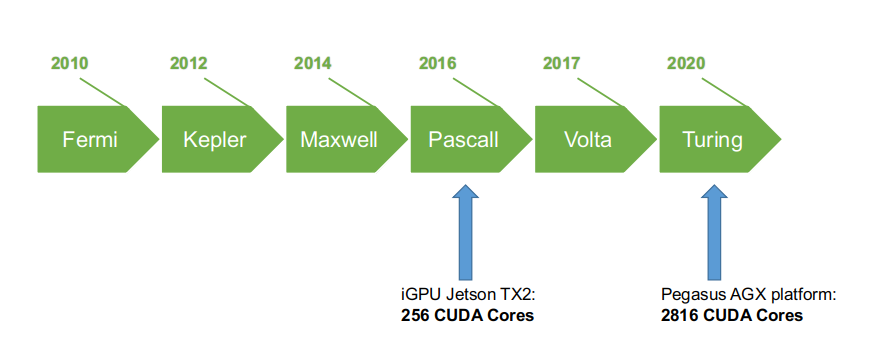
\includegraphics[scale=0.5]{Pictures/ch1/microarchitecture.png}
		\caption{CUDA micro-architectures over the years \label{fig:dagmapping}}
    \end{figure}  
    
	For example co-scheduling multiple pipelines together on the same GPU hardware would first require ascertaining the feasibility of scheduling independent kernels together since they share common memory. Thus, it becomes increasingly crucial to consider locality aware optimizations at the time of dispatching individual kernels to the GPU. 
	
	However, in order to understand the nuances of scheduling these optimized kernels, we must first understand the GPU architecture on which these kernels will be executed and the underlying programming model. Chapter 2 provides the necessary background context on CUDA, while Chapter 3 covers thread coarsening as an optimization along with discussion on the observations made over the course of the project.

   

% Chapter Template

\chapter{The CUDA Model} % Main chapter title

\label{Chapter2} % Change X to a consecutive number; for referencing this chapter elsewhere, use \ref{ChapterX}

\lhead{Chapter 2. \emph{The CUDA Model}} % Change X to a consecutive number; this is for the header on each page - perhaps a shortened title

%----------------------------------------------------------------------------------------
%	SECTION 1
%----------------------------------------------------------------------------------------

\section{Introduction}


CUDA is a parallel computing platform and programming model that serves as an extension to the C language. It allows development of applications for various kinds of devices, such as personal computers, embedded systems to HPC clustered systems.

In addition to sharing many abstractions with other parallel programming models, the CUDA programming model provides the following special features to harness the computing power of GPU architectures: 
\begin{itemize}
    \item A way to organize threads on the GPU through a hierarchy structure
    \item A way to access memory on the GPU through a hierarchy structure
\end{itemize}

Unlike C parallel programming, where the programmer is responsible for managing threads explicitly using either pthreads or OpenMP techniques, CUDA exposes a thread hierarchy abstraction which allows the programmer to control thread behavior.

\section{CUDA Programming Structure}

The CUDA programming model executes applications on a heterogeneous computing system, which comprises of two distinct program entitites:
\begin{itemize}
	\item \textbf{the host} - the CPU, and its memory (host memory)
	\item \textbf{the device} - The GPU, and its memory (device memory)
\end{itemize}


At the core of the CUDA programming model is the \textbf{kernel} - the code that runs on the GPU hardware. The CUDA model allows developers the freedom to write kernel as a sequential program - abstracting away the parallelism, and manages scheduling the developer-written code on the GPU threads. On the other hand, the host defines the mapping of the algorithm to the device based on parameters such as the application data and the GPU device capability. This model allows developers the benefit of focusing on the algorithm in a scalar fashion, by writing sequential code, and not get distracted by the details and nuances that often come up with creating and managing thousands of GPU threads.


Unless explicitly programmed by the programmer, the host operates independently of the device. When a kernel is launched by the host, the control returns to the host immediately, freeing the CPU to perform additional tasks while the kernel gets executed on the device. The CUDA programming model is asynchronous so the GPU computation happening on the GPU can be overlapped with the host-device communication.  A typical CUDA program consists of the serial host code complemented by the parallel code executing on the device. 

For every computational kernel, the single-threaded host program leverages command queues supported by the OpenCL API to issue commands for  performing the following operations: 

The processing flow in a standard CUDA program follows this sequence:
\begin{itemize}
	\item \textbf{Host to Device or H2D transfer} - copying the data from host to input buffers resident on device memory. 
	\item \textbf{Execution} - launching the kernel in a SIMD fashion on the target device.
	\item \textbf{Device to Host or D2H transfer} - copying back the data stored in output buffers in the device after the kernel has finished processing back to the host memory.
\end{itemize}

As the CUDA programming model assumes a system comprising of a host and a device, each with its separate memory, the model provides functions to allocate and release device memory. In addition, it also provides functions to transfer data between the host and the device memory. This directly follows the processing flow given in the preceding paragraph. The control over both device and host memory is especially important given that the kernels operate out of device memory, and therefore providing complete control over device memory management allows programmers to achieve the best performance.

Another interesting characteristic of the CUDA programming model is the exposed memory hierarchy. Each GPU device has different types of memory used for different purposes. The two main types of memories in any GPU device are the global and the shared memory. The global memory is analogous to the CPU system memory, while the shared memory is similar to the CPU cache. However, and perhaps quite notably, GPU shared memory can be directly controlled from a CUDA kernel.


\begin{figure}[ht]
	\centering
	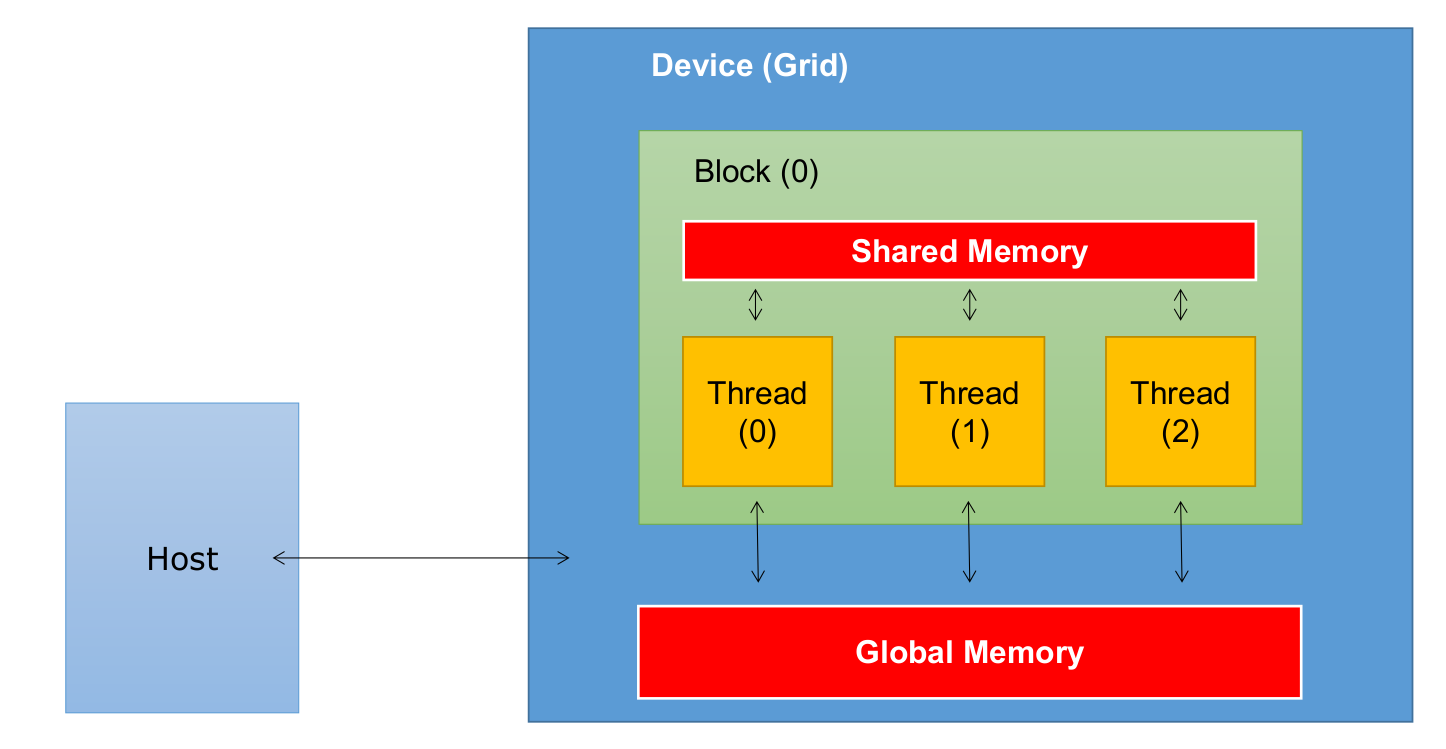
\includegraphics[scale=0.30]{Pictures/ch2/cuda_mem_hierarchy.png}
	\caption{\small CUDA memory hierarchy}
\end{figure}


% thread hierarchy
So far, we have discussed about the memory hierarchy in CUDA and how the different kinds of memory interact with the threads during the execution. The threads in CUDA themselves are organized in a two-tier hierarchy, which can be decomposed into 'blocks' of threads, and 'grids' of blocks.

Whenever a host program launches a kernel with a set number of threads, all threads belong to a single unit called the grid. All threads in a grid share the same global memory space as shown in figure 2.1. Each grid itself comprises of single (or multiple) blocks. A thread block is a localised group of threads which have more intimate cooperation with each other as they interact with each other using:

\begin{itemize}
    \item block-local synchronization
    \item block-local shared memory
\end{itemize}

Threads belonging to different blocks cannot cooperate. 
In order to navigate through this hierarchy and address each thread uniquely, CUDA employs two unique coordinates to distinguish threads:

\begin{itemize}
    \item \textbf{blockIdx}: block index within a grid
    \item \textbf{threadIdx}: thread index within a block
\end{itemize}

These variables are built-in and pre-initialized that can be directly accessed within a kernel. During the kernel execution, the coordinate variables are assigned to each thread automatically by the CUDA runtime. By assigning conditions on the values of these variables, portions of data can be assigned to different threads.

The coordinate variable is of type \textit{uint3}, a CUDA built-in vector type, derived from the basic integer type. It is a structure containing three unsigned integers, and the 1st, 2nd, and 3rd components are accessible through the fields x, y, and z respectively:

% \usepackage{minted}

% \begin{document}
% \begin{minted}{python}
\textit{threadIdx.x    blockIdx.x} \newline
\textit{threadIdx.y    blockIdx.y} \newline
\textit{threadIdx.z    blockIdx.z}

\begin{figure}[ht]
	\centering
	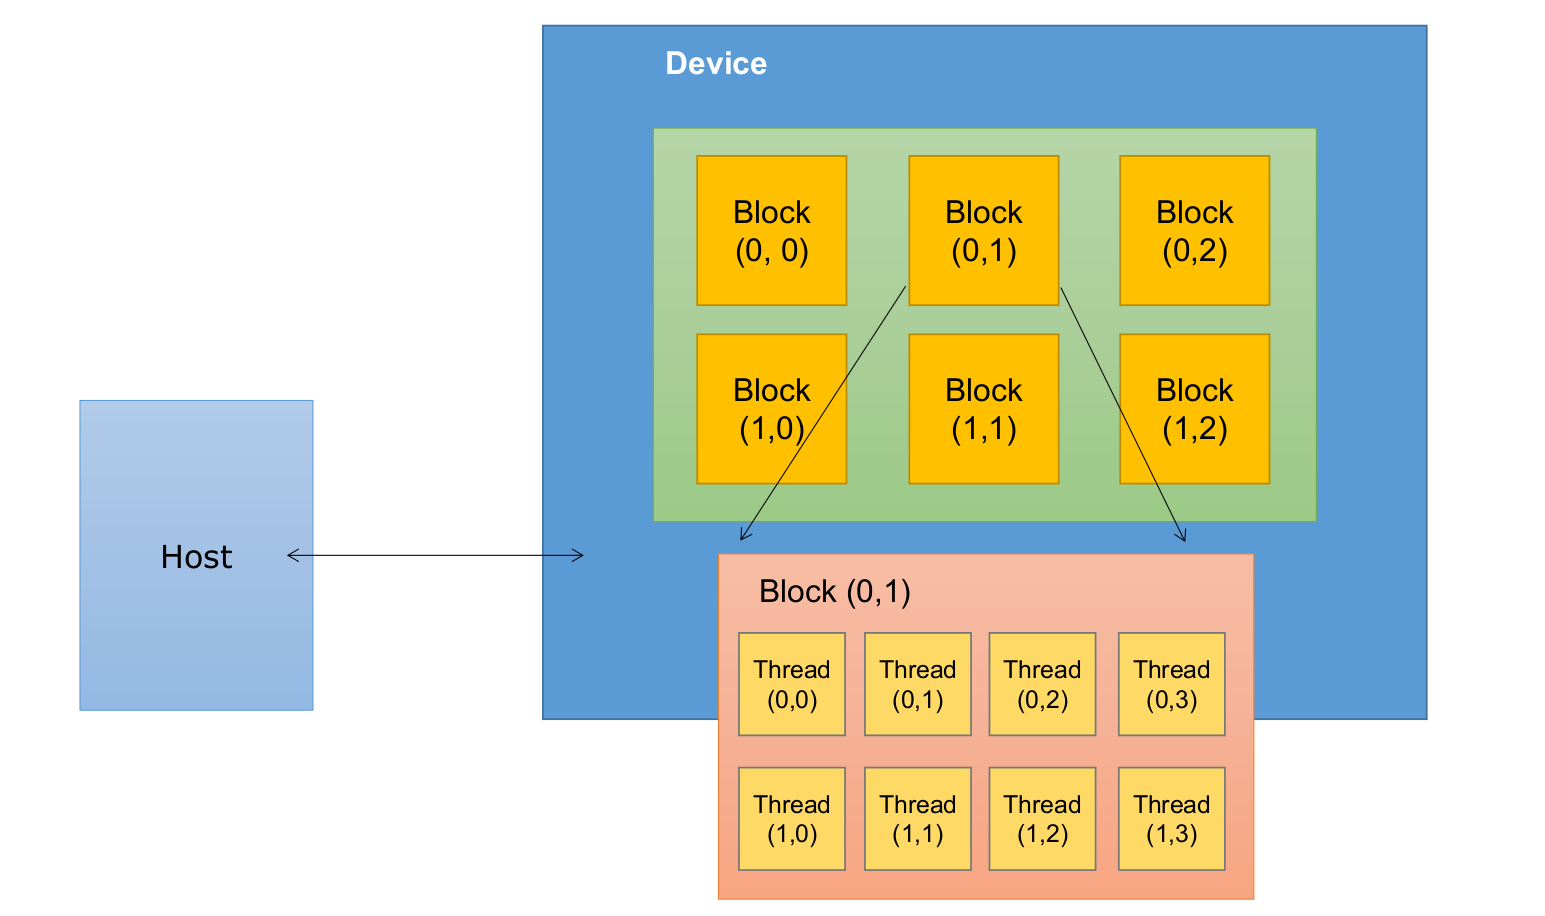
\includegraphics[scale=0.30]{Pictures/ch2/cuda_thread_hierarchy.png}
	\caption{\small CUDA thread hierarchy}
\end{figure}

% threadIdx.x blockIdx.x \newline
% threadIdx.y blockIdx.y
% \end{minted}
% \end{document}

\section{An Example}

	\par As an illustrative example, we consider a simple CUDA application which performs a vector addition. The vector addition kernel $vadd$ executes on device $GPU_0$. It takes as input two input buffers ($in1$ and $in2$) performs element-wise addition and produces an output buffer ($out$). In Fig. \ref{fig:OpenCLArch}, the CUDA host program sets prepares for kernel execution by transfering the input data from the host memory to the device memory through the cudaMemcpy(..cudaMemcpyHostToDevice) instruction. Once the input buffers have been transferred to the device memory, the kernel $addVectors$ is launched with some block and grid dimensions. The mapping is done such that each thread in a thread block would compute exactly one element in the output vector. It is possible, however, that the final block might have some threads which do not map to any element in the output vector (due to block size not being a factor of size of vectors). In this case, threads which are not necessary are disabled through a preliminary if condition in the kernel code.
	
	The kernel code simply calculates the unique global ID of each thread, and computes the corresponding output element with the index equal to the global ID of the thread. The expression $int id = blockIdx.x * blockDim.x + threadIdx.x$ calculates the index of the current thread in the entire grid, which allows us to uniquely identify this thread within the entire grid, and not just the block through a single number.
	
	The kernel execution is completed when all thread blocks finish execution. At this point, the resulting vector $out$ is ready to be copied from the device memory back to the host memory. This is again done using the cudaMemcpy() function except this time we use the cudaMemcpyDeviceToHost object to signal that data is being transferred from device to host this time.
	
	\begin{figure}[ht]  
		\centering
		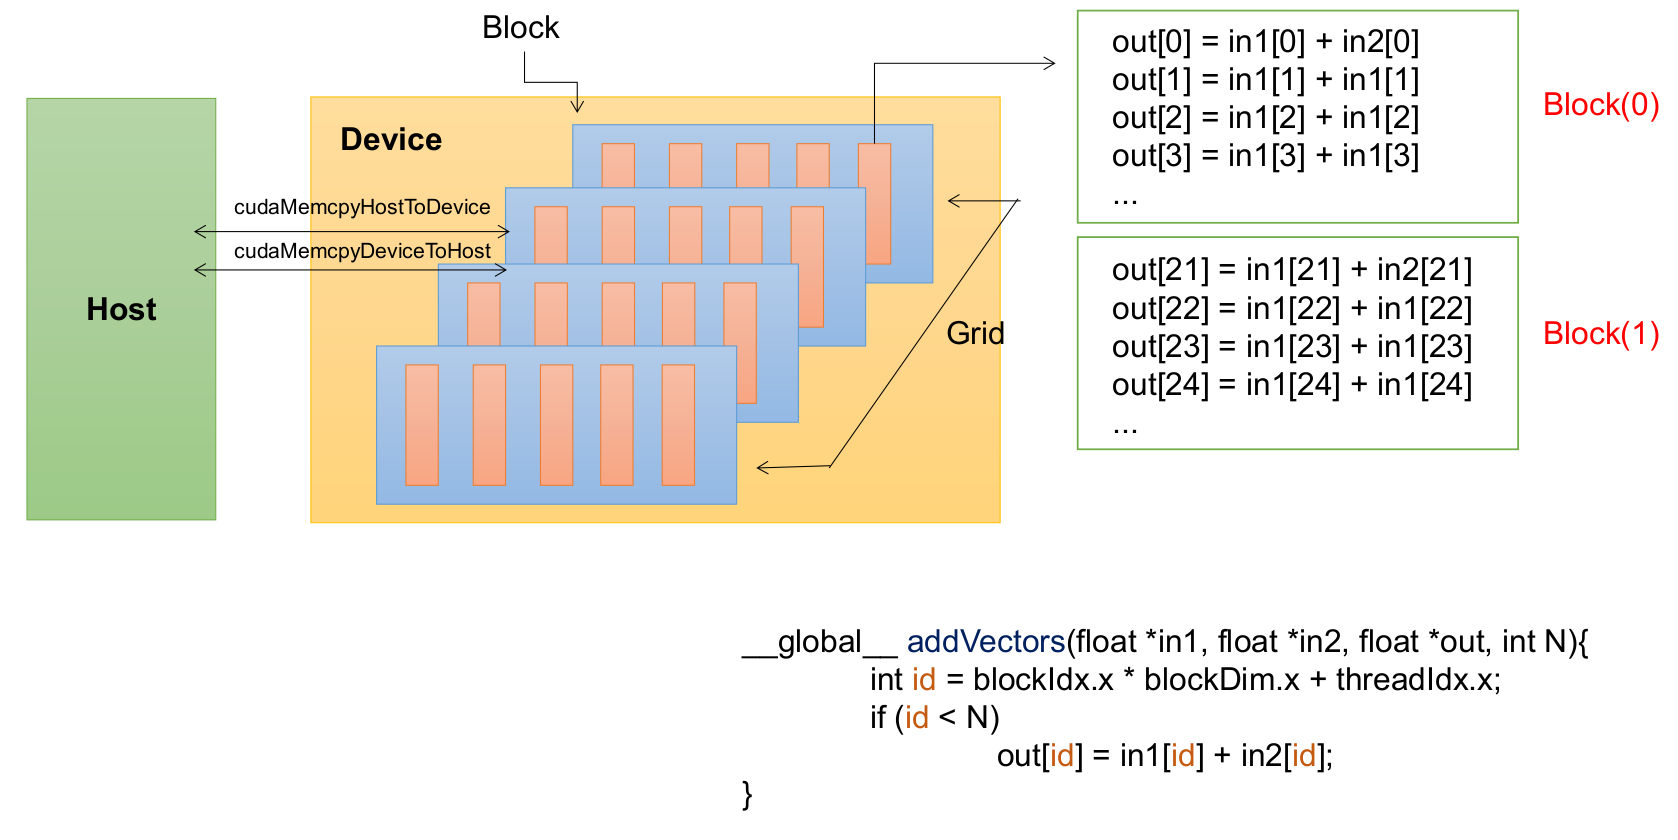
\includegraphics[scale=0.25]{Pictures/ch2/add_example.png}
		\caption{OpenCL Execution \label{fig:OpenCLArch}}
	\end{figure}
	
	However, as explained previously, the host and device are asynchronous, and the control returns back to the host program as soon as the kernel is launched on the device. Therefore, if there is no barrier in place, the control reaches the cudaMemcpy instruction immediately. This might result in incorrect data being copied from the device to host as there is a chance that the kernel execution has not yet finished. This issue was identified by the CUDA developers early on, and therefore, the cudaMemcpy function was thus converted into one of the few synchronous functions in the CUDA library. This ensured that the copy instruction was not executed before the device finished executing the kernel. 
% Chapter Template

\chapter{Thread Coarsening} % Main chapter title

\label{Chapter3} % Change X to a consecutive number; for referencing this chapter elsewhere, use \ref{ChapterX}

\lhead{Chapter 3 \emph{Thread Coarsening}} % Change X to a consecutive number; this is for the header on each page - perhaps a shortened title

\section{What is coarsening?} \label{sec:what_is_coarsening}
Thread coarsening is an optimization technique that is often employed in GPU kernels, wherein the code that is meant to be executed by a larger number of threads gets merged into a single thread; which leads to launching fewer but more coarse-grained threads.

The nature of thread coarsening is such that it leads to a reduction in parallelism by reducing the number of threads being launched. This can, depending on the type of work being done by the kernel and the extent to which the threads are being coarsened, have a beneficial or a detrimental effect on the execution time of the kernel. To coarsen a kernel, say by a factor of 2, all instructions dependent on the thread index are duplicated, while the rest of the instructions are shared between the two coarsened instances within the kernel. These shared instructions include the CUDA API's synchronization barrier, '\_\_syncthreads()', which features quite commonly in the convolution kernels employing shared memory optimizations.

\begin{figure}[ht]
	\centering
	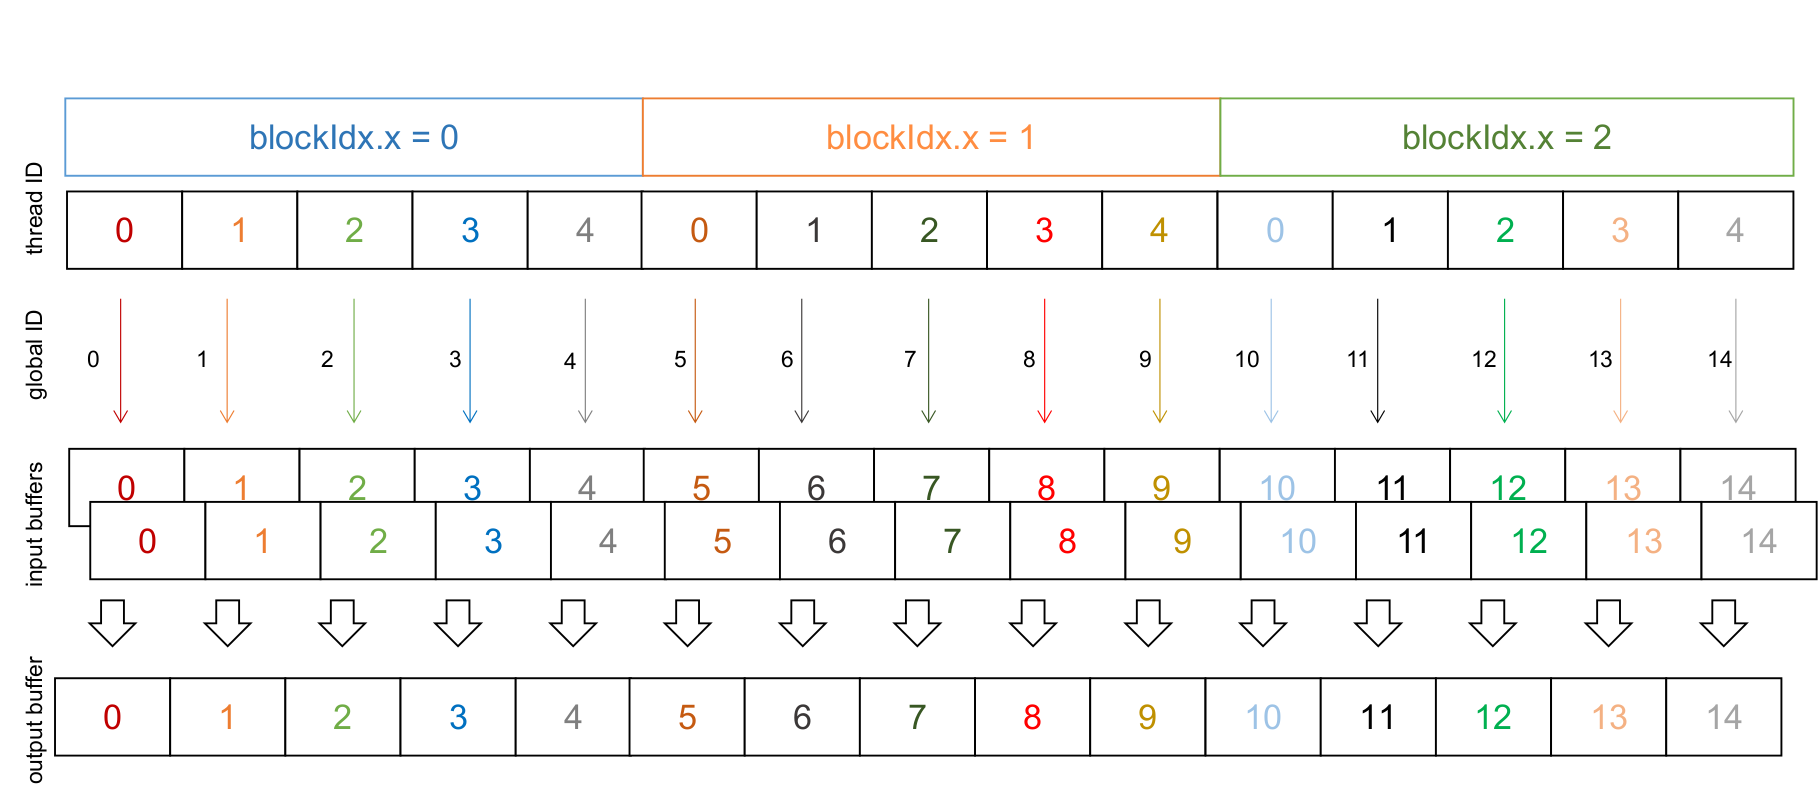
\includegraphics[scale=0.25]{Pictures/ch3/thread_allocation.png}
	\caption{\small CUDA thread mapping}
\end{figure}


\begin{figure}[ht]
	\centering
	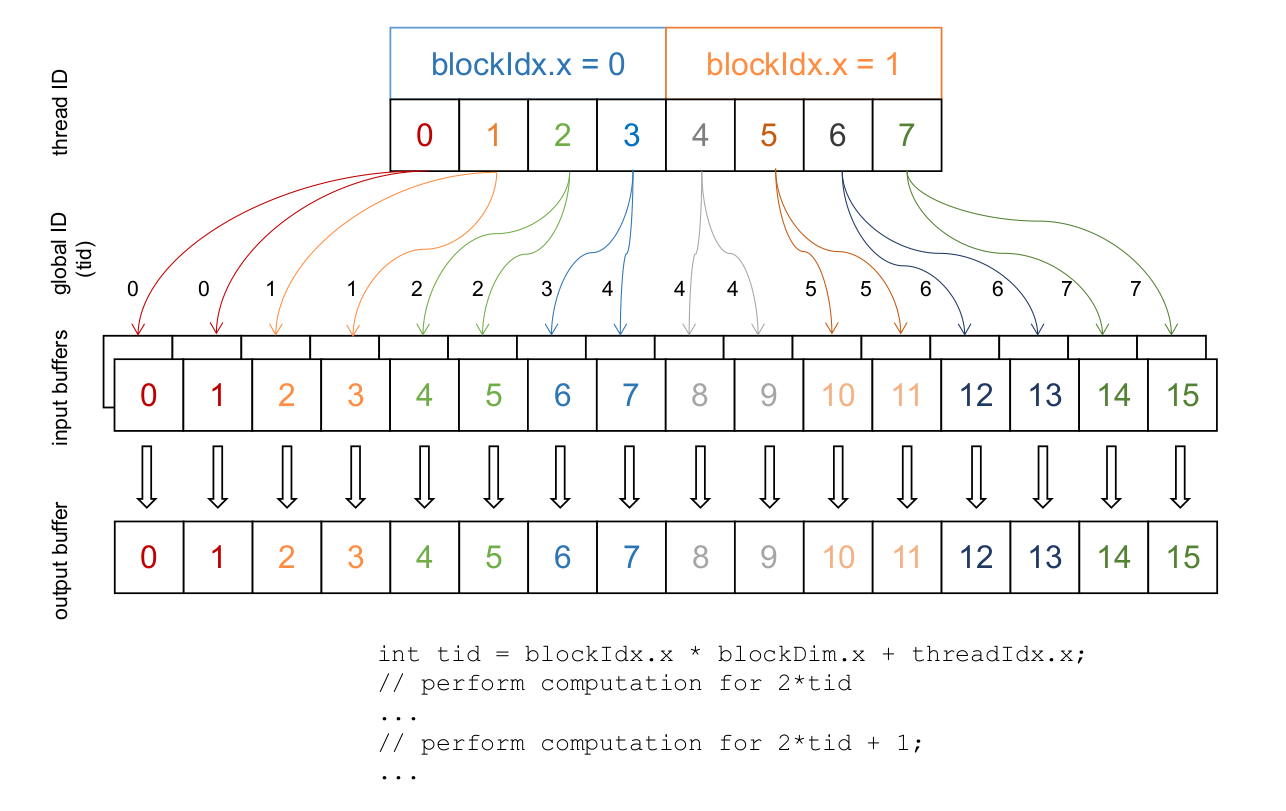
\includegraphics[scale=0.35]{Pictures/ch3/coarsen_2C2S.png}
	\caption{\small CUDA thread coarsening for C = 2, S = 2}
\end{figure}

\begin{figure}[ht]
	\centering
	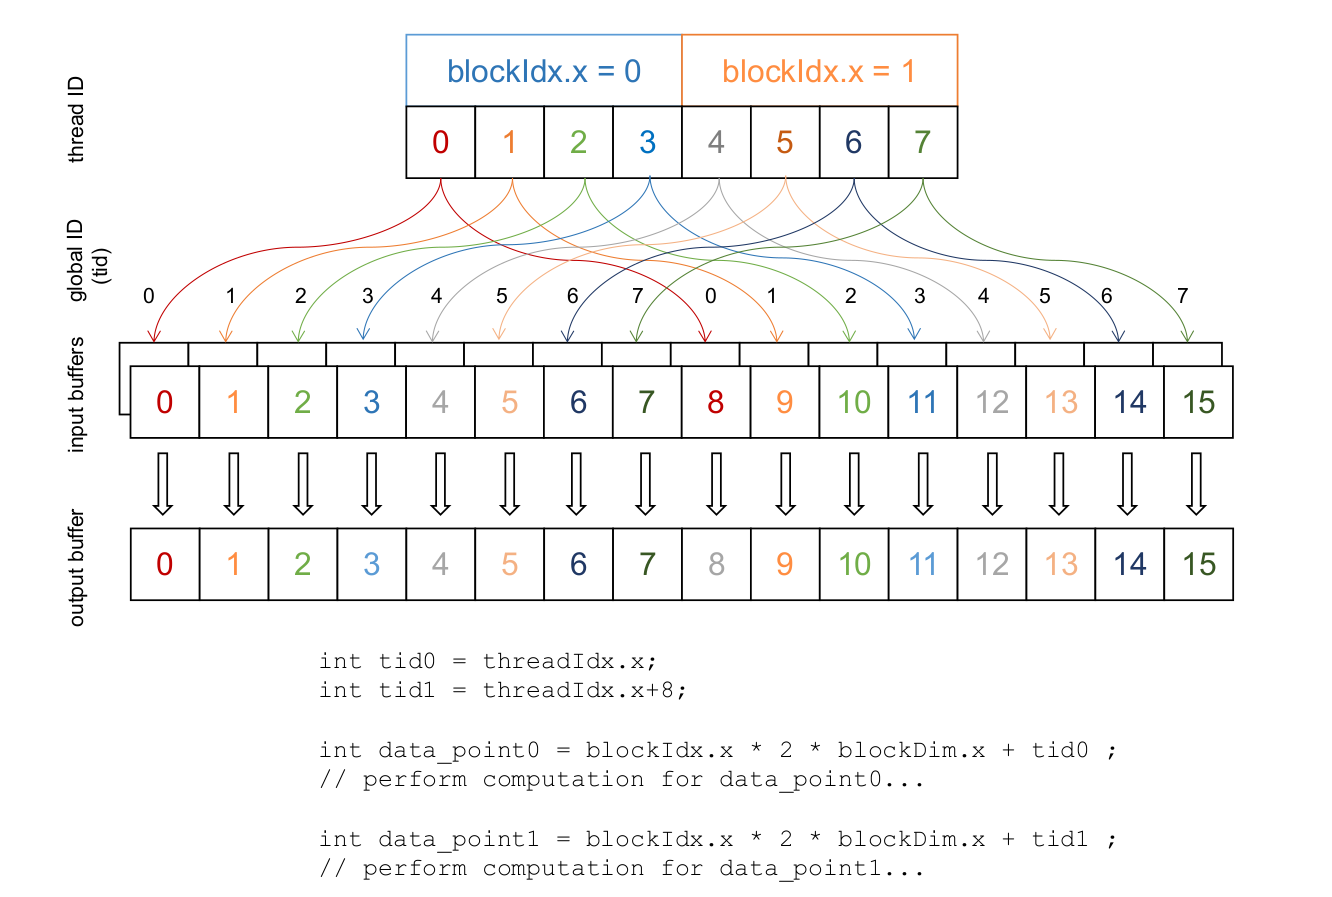
\includegraphics[scale=0.35]{Pictures/ch3/coarsen_2C8S.png}
	\caption{\small CUDA thread coarsening for C = 2, S = 8}
\end{figure}


\begin{figure}[ht]
	\centering
	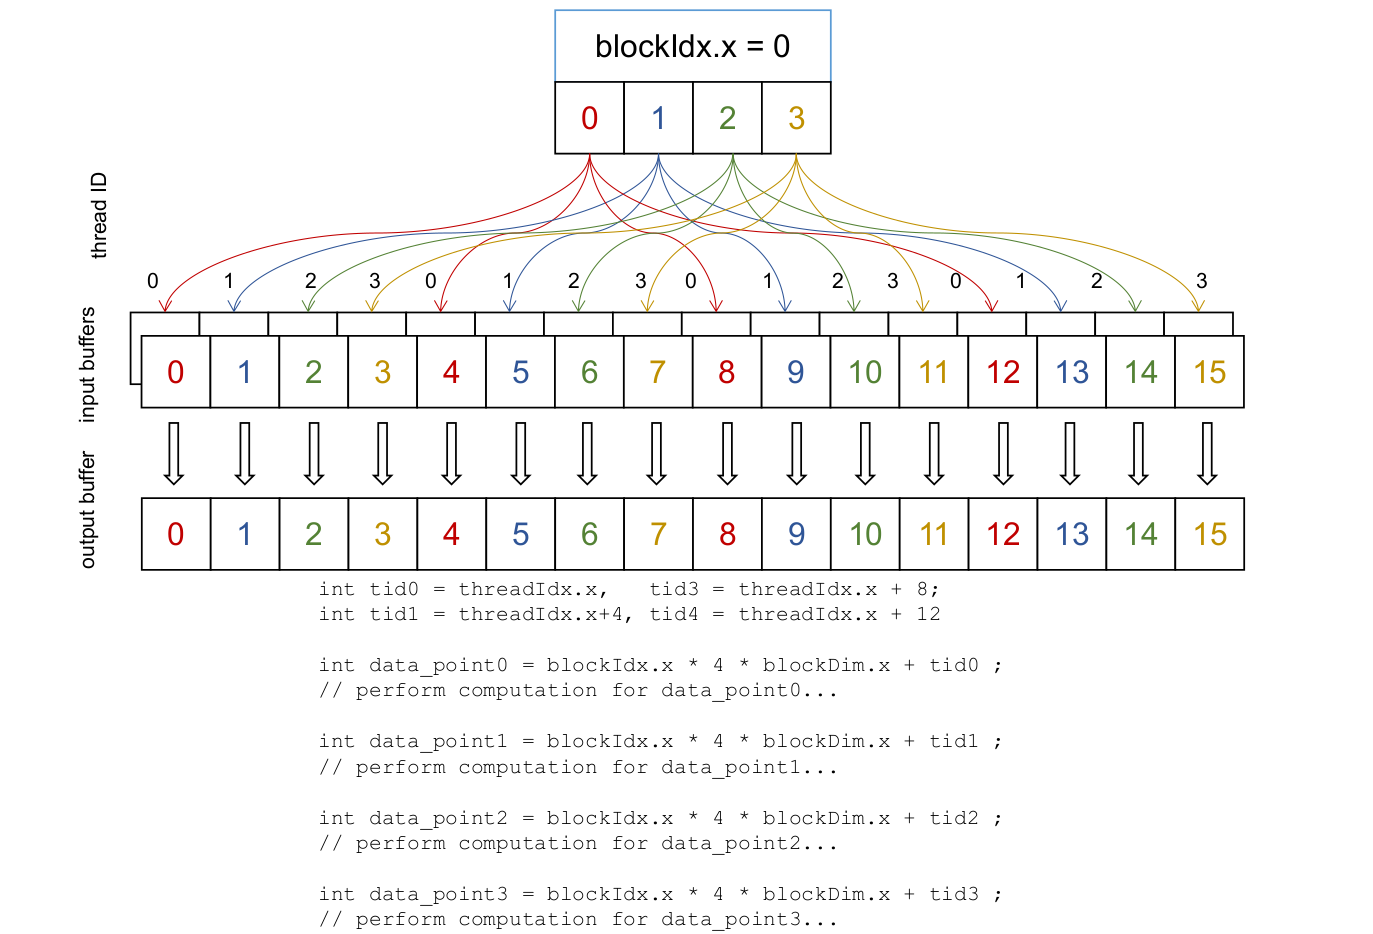
\includegraphics[scale=0.35]{Pictures/ch3/coarsen_4C4S.png}
	\caption{\small CUDA thread coarsening for C = 4, S = 4}
\end{figure}

\section{Effects of coarsening} \label{sec:effect_of_coarsening}

Thread coarsening, by the virtue of being an optimization technique, allows programmers to maximize GPU utilization, and reduce the execution-time of kernels. However, as mentioned in the preceding section, this can, depending on several factors, also lead to a decrease in the parallelism, and consequently, the performance of the kernel. In this work, I have tried to better understand and provide a theoretical justification to the performance changes we see in the convolution kernels when coarsened to different extents.

To understand how coarsening affects kernels and try and predict whether coarsening might be helpful for a given convolution kernel with fixed hyper-parameters, we first need to understand the broad changes that are introduced when a kernel is coarsened.

The biggest, and perhaps the most evident change brought by coarsening is the reduction in the number of threads that are launched to finish the execution of the code. As each thread now performs the work that was previously done by multiple threads, the number of threads launched reduces by a factor of the number of threads whose work is fused into one, more commonly known as the coarsening factor. Thus, for a convolution kernel coarsened by a factor of 8, if the original kernel was launched with 256 threads; the coarsened kernel will be launched with only 32 threads.

This reduction in the size of thread block being launched for a kernel leads to an improvement in the kernel execution time in primarily three ways:

i. smaller thread blocks lead to a greater number of concurrent blocks being scheduled on the same SM, which reduces the number of batches that need to be executed to complete the computation. This leads to an improvement by cutting down on the overhead that accompanies scheduling and executing thread blocks on the SM.

ii. fewer number of threads launched leads to a lesser number of barrier calls made, taken over the entire execution of the program

iii. greater number of instructions per thread leads to better exploitation of hardware instruction-level parallelism.

One would expect these advantages to scale with the coarsening factor, which they do to some extent. As the level of coarsening increases, we eventually reach a point where the reduction in parallelism due to the extensive coarsening can no longer be compensated for by the advantages mentioned above. From this point on, any further attempts at coarsening the kernel only lead to a decrease in the observed performance.  

In addition to this reduction in parallelism, the coarsened threads are also more resource-hungry. As the work being done by the threads in a coarsened kernel is more, it raises the thread block's resource requirements, such as the number of registers and shared memory needed, which in turn lead to a reduced occupancy. Thus, when it comes to thread coarsening, there is a very clear performance tradeoff at play, and the problem of identifying the optimal coarsening factor (or deciding no coarsening is beneficial) for a given kernel is still a non-trivial problem.

In the next section, we will compare the performance of a convolution kernel against itself when coarsened to different extents, and try to provide some theoretical justification to the results observed.

\section{Results \& Observations} \label{sec:predict_coarsening}

The first part of the project done in this semester deals with the implementation of a single parameterized pass that can automatically coarsen convolution kernels with a user-defined value of coarsening factor and stride, and generate the CUDA code for the same. This was implemented using a macro processor known called PyExpander, which allows Python code to be embedded in text files. Coarsening by definition involves repetition of instructions which are dependent on thread indices. Thus, for a given convolution kernel, the script uses loops in the text file to replicate the relevant statements.

\begin{figure}[ht]
	\centering
	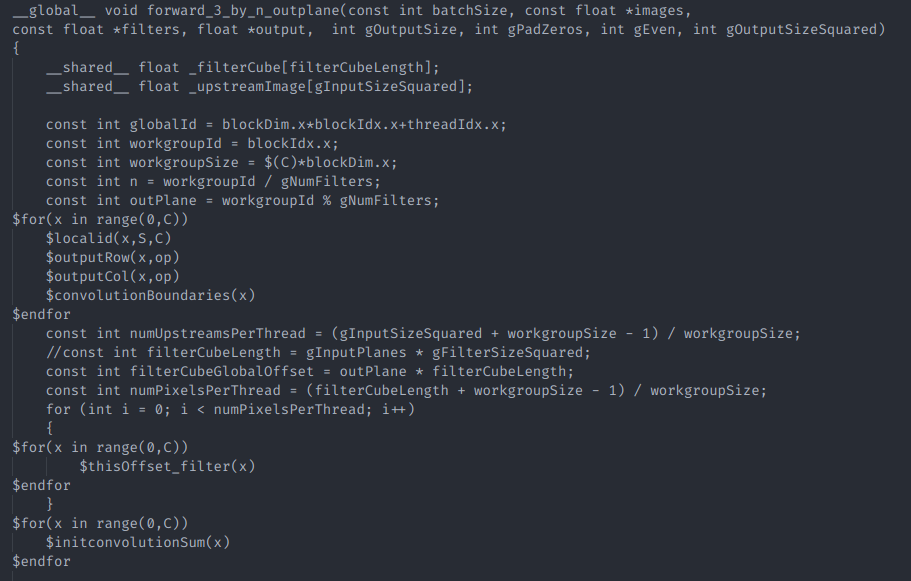
\includegraphics[scale=0.45]{Pictures/ch3/script.png}
	\caption{\small PyExpander script for generating coarsened kernels}
\end{figure}

Such a script allows generation of coarsened kernels with custom coarsening factors, which is vital in the development of the CUDA scheduler that determines optimal coarsening factors depending on the available hardware resources at any moment. This serves an important purpose of not having to generate the coarsened kernels for different values of C prior to kernel launch, and more importantly, provides the system with the flexibility to determine an appropriate coarsening factor without any constraints on the values allowed.

\begin{figure}[ht]
	\centering
	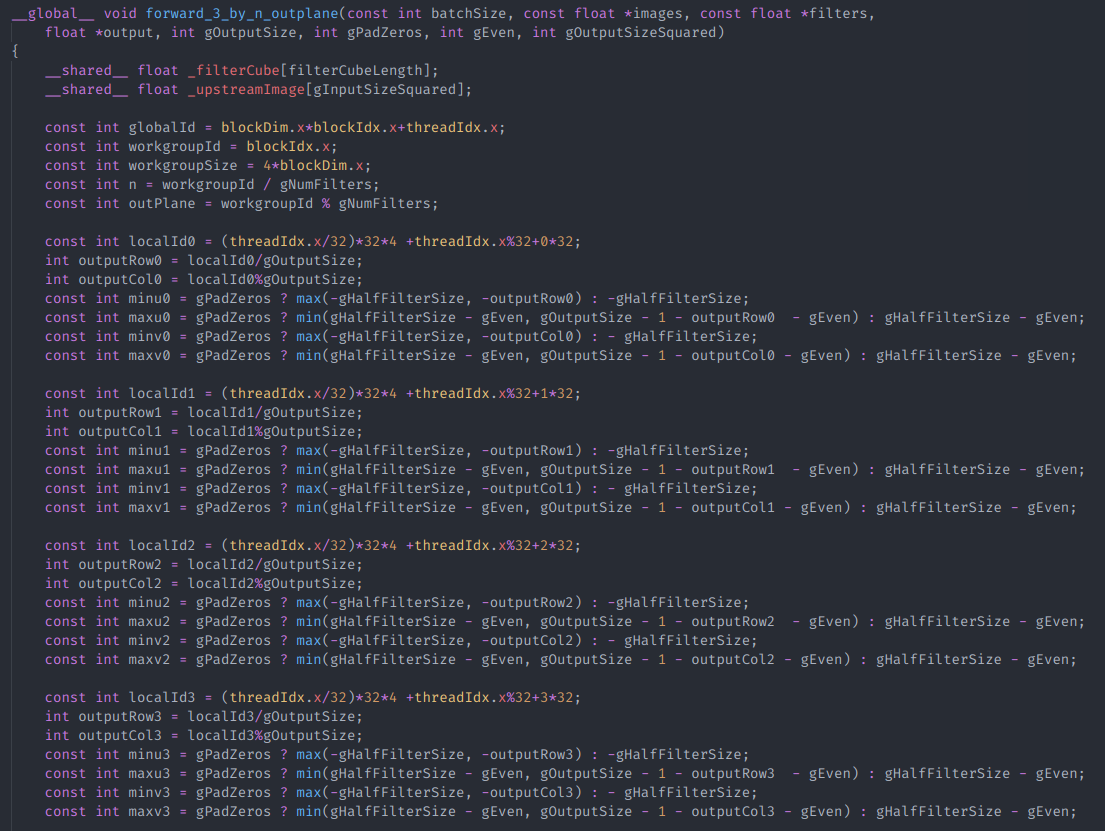
\includegraphics[scale=0.4]{Pictures/ch3/code coarsened.png}
	\caption{\small Coarsened convolution kernel for C=4}
\end{figure}


As mentioned in the preceding section, the effects of thread coarsening are not uniform and instead depend on the kernel being coarsened. For our specific problem, focused on CNN pipelines and attempting to coarsen the convolution kernels, the difference in kernels arise from the changes in hyper-parameters such as the size of the input, number of channels in the input input, number of filters, etc. Simply modifying these hyper-parameters without changing any other part of the kernel code can significantly alter the behavior changes we see due to coarsening in the kernel. To study the effects of coarsening and try to justify them, we will first limit ourselves to a specific set of hyper-parameters values and observe the results when this kernel is coarsened using different coarsening factors.


The kernel we are going to analyse is a 3D convolution kernel, which computes performs convolution of multiple images in a batch with a given filter in a single pass. The kernel is optimized by making use of shared memory for faster repeated read operations while performing the convolution. The hyper-parameters for this experiment are as follows:

\begin{itemize}
\item batch size: 1024
\item size of single channel in input image: 31 x 31
\item number of channels in input image: 5
\item size of single channel in input filter: 3 x 3
\item number of filters: 2
\end{itemize}

The speedups for this kernel's coarsened variants are given in table 3.1, and visualised in fig 3.7

% \begin{table}[ht]
%     \centering
    
%     \begin{tabular}{ |p{5cm}|p{5cm}|  }
%          \hline
%          Coarsening factor & Execution time (in ms) \\
%          \hline
%          1 (Uncoarsened)    & 1.66\\
%          2                  & 1.09\\
%          4                  & 0.91\\
%          8                  & 1.08\\
%          16                 & 1.58\\
%          32                 & 5.73\\
%          \hline
%     \end{tabular}
%     \caption{\small Execution times for different coarsening factors}
%     \label{tab:execution_time_good_coarsen}
% \end{table}

\begin{figure}[ht]
	\centering
	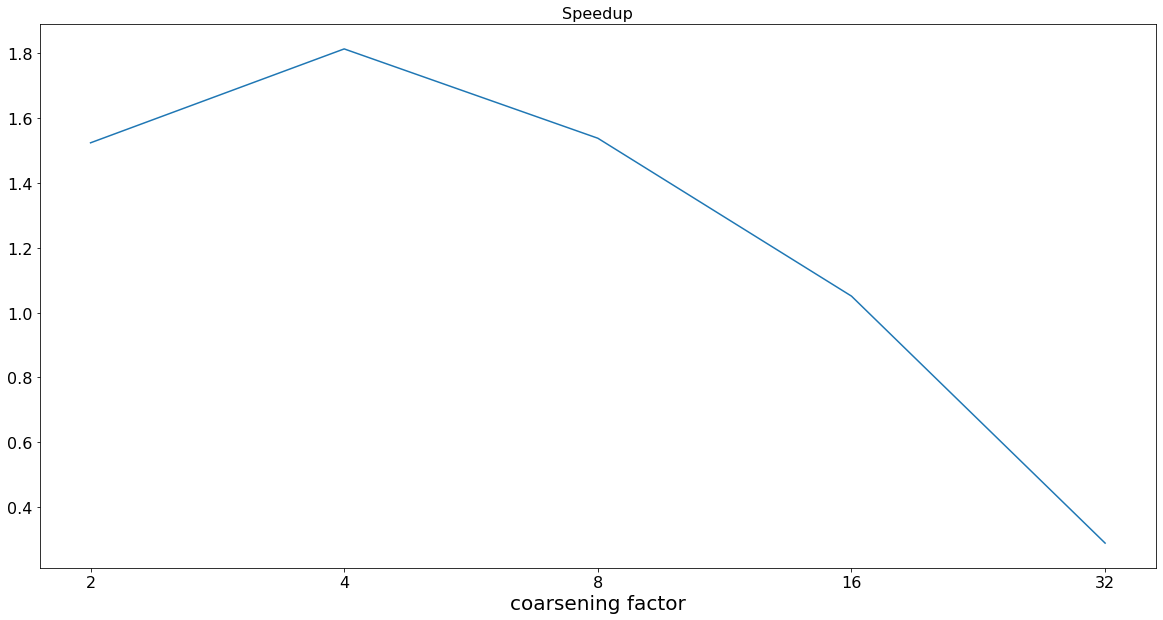
\includegraphics[scale=0.30]{Pictures/plots/good_improvement_coarsening/speedup.png}
	\caption{\small Speedup for differently coarsened kernels - Case I}
\end{figure}

A cursory look at the data seems to match the hypothesis we had established so far of decreased execution time with increase in the coarsening factor till a limit (in this example, that limit is 4), following which the performance starts degrading rapidly.

In order to justify this behavior, let us also look at the block size in each of these cases from table 3.1.

% \begin{table}[ht]
%     \centering
    
%     \begin{tabular}{ |p{5cm}|p{5cm}|  }
%          \hline
%          Coarsening factor & Thread block size \\
%          \hline
%          1 (Uncoarsened)    & 841\\
%          2                  & 448\\
%          4                  & 224\\
%          8                  & 128\\
%          16                 & 64\\
%          32                 & 32\\
%          \hline
%     \end{tabular}
%     \caption{\small Size of thread blocks for different coarsening factors}
%     \label{tab:block_size_good_coarsen}
% \end{table}

The maximum number of resident threads allowed on an SM at any given time, for the hardware on which these experiments were conducted, is 2048. Therefore, following the size of thread blocks as given in table 3.1, we see that the reduction in the size of thread block allows for more blocks to be scheduled and executed concurrently on the SMs. This reduces the number of batches for which execution needs to be performed, as more data is now being processed per batch, which in turn leads to a decrease in the execution time due to the overhead associated with scheduling and execution of batches in the SM. However, as table 3.1 also makes very evident, this justification does not extend beyond a coarsening factor of 4, at which point onward, even with a decrease in the size of the thread block, the execution time starts to rise.

To understand this behavior, we need to introduce another metric in our analysis, the register pressure. As the kernel is coarsened, and number of threads reduces, each individual thread performs more instructions, and in turn requires greater number of registers to execute. The number of registers required per thread to execute the kernel is known as the register pressure, or the registers per thread. For the kernel under consideration, the register pressure varies as seen in figure 3.8.

\begin{figure}[ht]
	\centering
	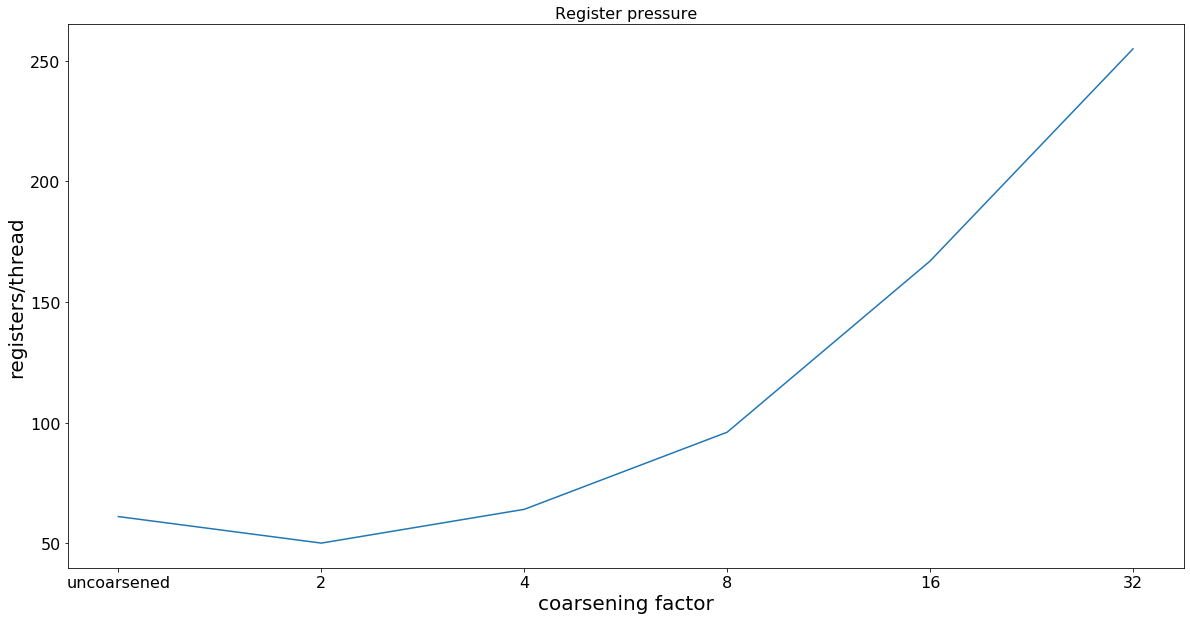
\includegraphics[scale=0.30]{Pictures/plots/good_improvement_coarsening/register pressure.png}
	\caption{\small Register for differently coarsened kernels - Case I}
\end{figure}

% \begin{table}[ht]
%     \centering
    
%     \begin{tabular}{ |p{5cm}|p{7cm}|  }
%          \hline
%          Coarsening factor & Register pressure (registers/thread) \\
%          \hline
%          1 (Uncoarsened)    & 61\\
%          2                  & 50\\
%          4                  & 64\\
%          8                  & 96\\
%          16                 & 167\\
%          32                 & 255\\
%          \hline
%     \end{tabular}
%     \caption{\small Register pressure for different coarsening factors}
%     \label{tab:block_size_good_coarsen}
% \end{table}

Apart from the anomaly seen when going from an uncoarsened kernel to a coarsening factor of 2, the register pressure shows a regular trend with the decrease in the number of threads launched. With increase in the coarsening factor, each thread is responsible for carrying out more instructions, which is seen as an increase in the register pressure. For coarsening factor of 32, the register pressure exceeds the maximum hardware limit of 255, and the remaining registers are accessed from the global memory, a phenomenon known as register spilling.

An increased register pressure implies a greater resource demand for each warp scheduled on the SM. As the resources available on any SM are limited, this in turn leads to another potential parameter which could act as a bottleneck in terms of scheduling and execution of thread blocks. For the hardware used for this experiment, the number of registers present in an SM is 65,536. From table 3.1, for kernel with coarsening factor of 4, this would correspond to a maximum of 65,536/(32*64) = 32 warps concurrently scheduled warps in an SM. On the other hand, for coarsening factor of 8 and register pressure of 96, this number reduces to 65,536/(96*32), or just 21 active warps per SM. The theoretical (and the achieved) occupancy, therefore, are determined not just by one but multiple factors as demonstrated in this section. Apart from register pressure, other parameters such as shared memory per block can also act as a potential bottleneck. However, in our experiment, the amount of static shared memory per block does not change with the coarsening factor and therefore, can be ignored for purposes of evaluating change in the performance levels with different extents of coarsening. 

The results presented above can be in a summarised in a table as follows. In addition to the execution time and register pressure, we have also provided the theoretical and achieved occupancy for each of the cases, along with the \% utilization of the SM (on average) for each case.


\begin{table}[ht]
    \centering
    
    \begin{tabular}{ |p{2cm}|p{1.5cm}|p{1.5cm}|p{2cm}|p{2cm}|p{2cm}|p{2cm}|  }
         \hline
         Coarsening factor & Block size & Register pressure & Theoretical Occupancy & Achieved Occupancy & SM Utilization & Execution time (in ms) \\
         \hline
         
         1    & 841 & 61 & 84.38 & 83.32 & 43.44 & 1.66\\
         2                  & 448 & 50 & 87.5 & 85.96 &62.26 &  1.09\\
         4                  & 224 & 64 & 87.5 & 86 & 69.98 & 0.91\\
         8                  & 128 & 96 & 62.5 & 61.42 & 63.91 & 1.08\\
         16                 & 64 & 167 & 37.5 & 34.26 & 41.51 & 1.58\\
         32                 & 32 & 255 & 25 & 24.13 & 23.99 & 5.73\\
         \hline
    \end{tabular}
    \caption{\small Comparison of occupancy and execution time variation with coarsening factor - Case I}
    \label{tab:block_size_good_coarsen}
\end{table}



\begin{figure}[ht]
	\centering
	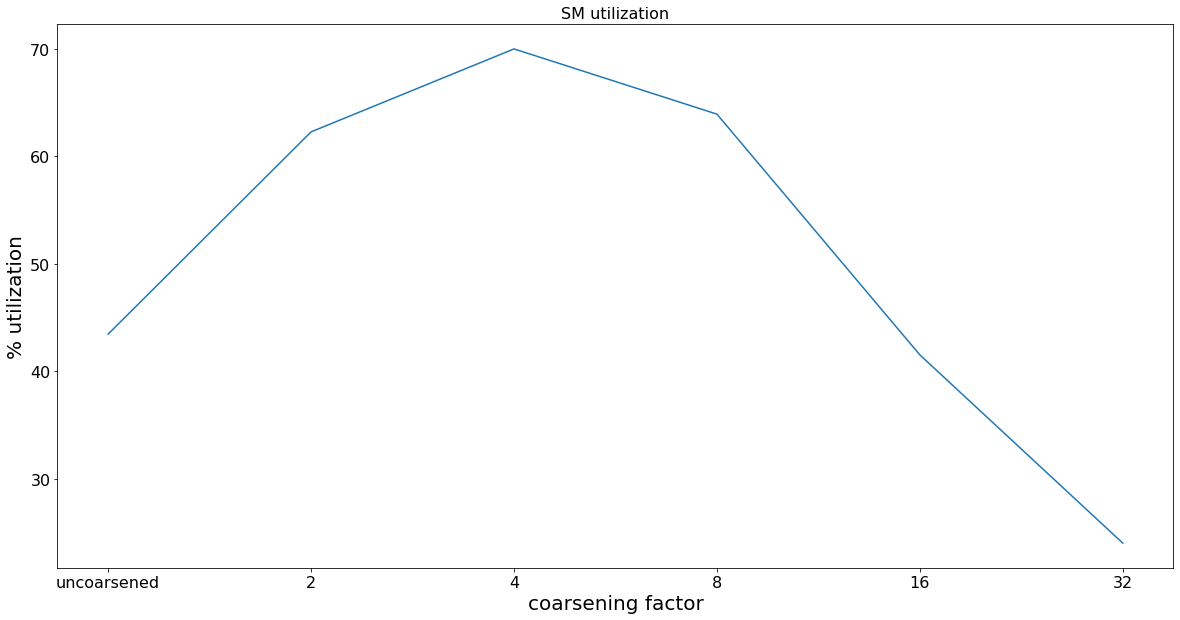
\includegraphics[scale=0.30]{Pictures/plots/good_improvement_coarsening/sm util.png}
	\caption{\small SM utilization for differently coarsened kernels - Case I}
\end{figure}

\begin{figure}[ht]
	\centering
	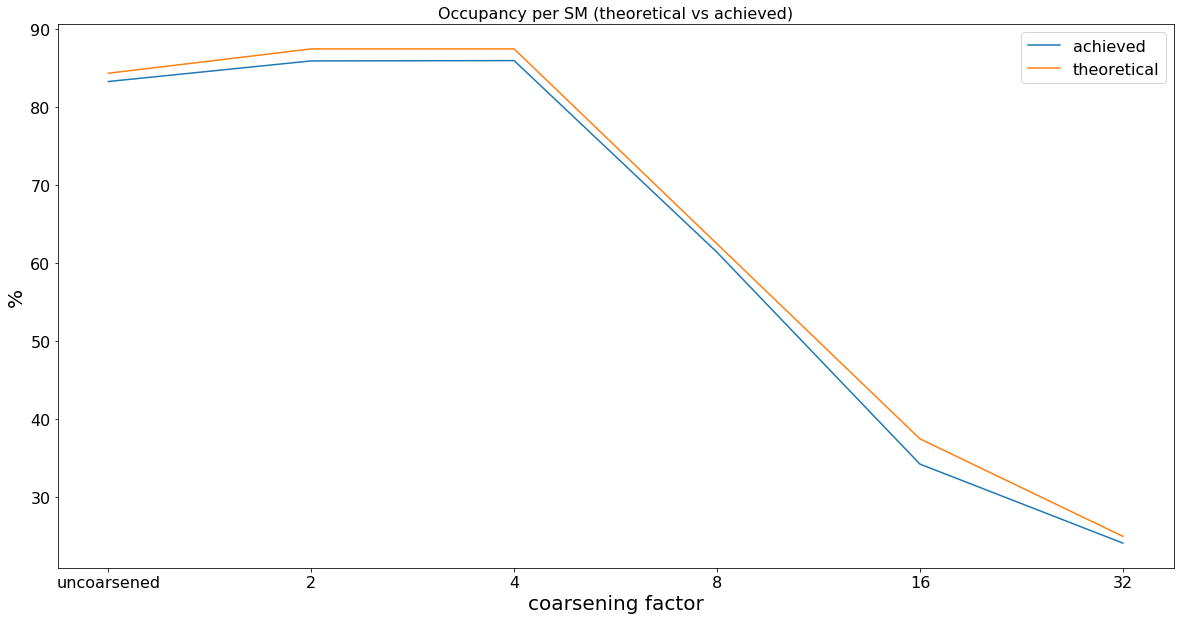
\includegraphics[scale=0.30]{Pictures/plots/good_improvement_coarsening/occupancy.png}
	\caption{\small Occupancy for differently coarsened kernels - Case I}
\end{figure}


Let us now consider the same convolution kernel with a different set of hyper-parameters where coarsening leads to a different trend in the variation of performance:


\begin{itemize}
\item batch size: 1024
\item size of single channel in input image: 45 x 45
\item number of channels in input image: 5
\item size of single channel in input filter: 15 x 15
\item number of filters: 2
\end{itemize}

The execution time for this kernel and the different coarsened variants is given below:

\begin{figure}[ht]
	\centering
	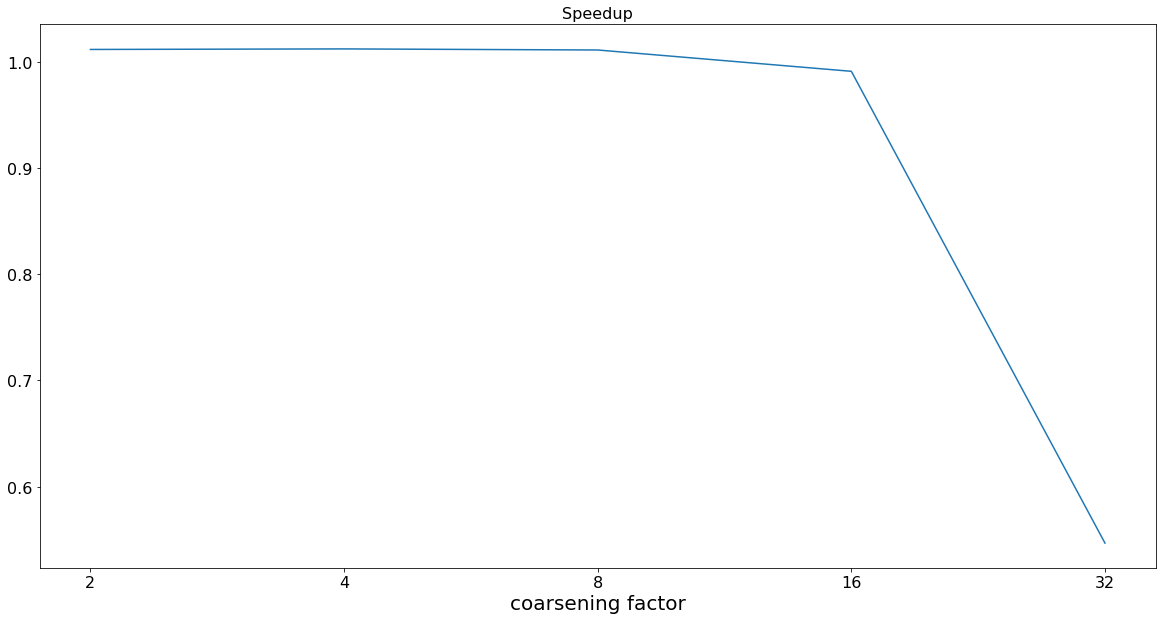
\includegraphics[scale=0.30]{Pictures/plots/poor_improvement/speedup.png}
	\caption{\small Speedup for differently coarsened kernels - Case II}
\end{figure}

In contrast to figure 3.7, we see that the speedup for this kernel isn't significant at all. While smaller coarsening factors ( less than 16 ) barely show any improvement in performance in terms of the execution time, further coarsening leads to a sharp degradation instead.

In order to understand this seemingly strange behavior, let us first observe the trend in occupancy because of the coarsening.

\begin{figure}[ht]
	\centering
	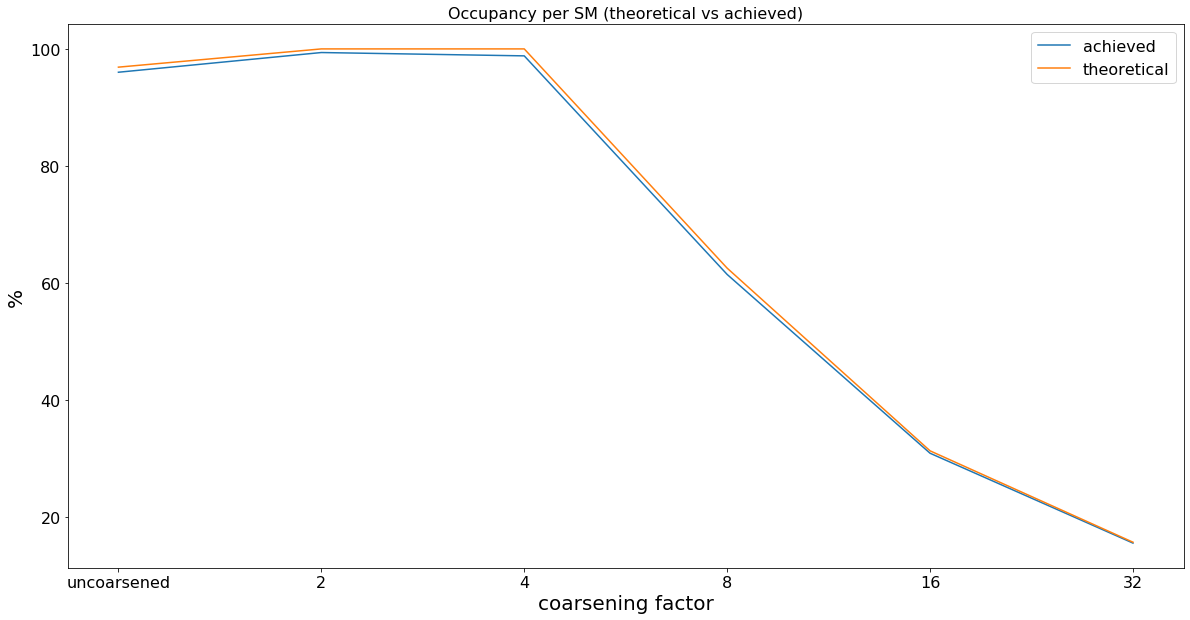
\includegraphics[scale=0.30]{Pictures/plots/poor_improvement/occupancy both.png}
	\caption{\small Occupancy for differently coarsened kernels - Case II}
\end{figure}

As one would expect after looking at the speedups, the occupancy does not change in any significant manner for small coarsening factors. However, for large coarsening factors, it shows a sharp decline and quickly falls off to sub-optimal levels.

Similar to the previous case, let us again try and see if the register pressure can tell us something about the observations for this case from figure 3.13.

\begin{figure}[ht]
	\centering
	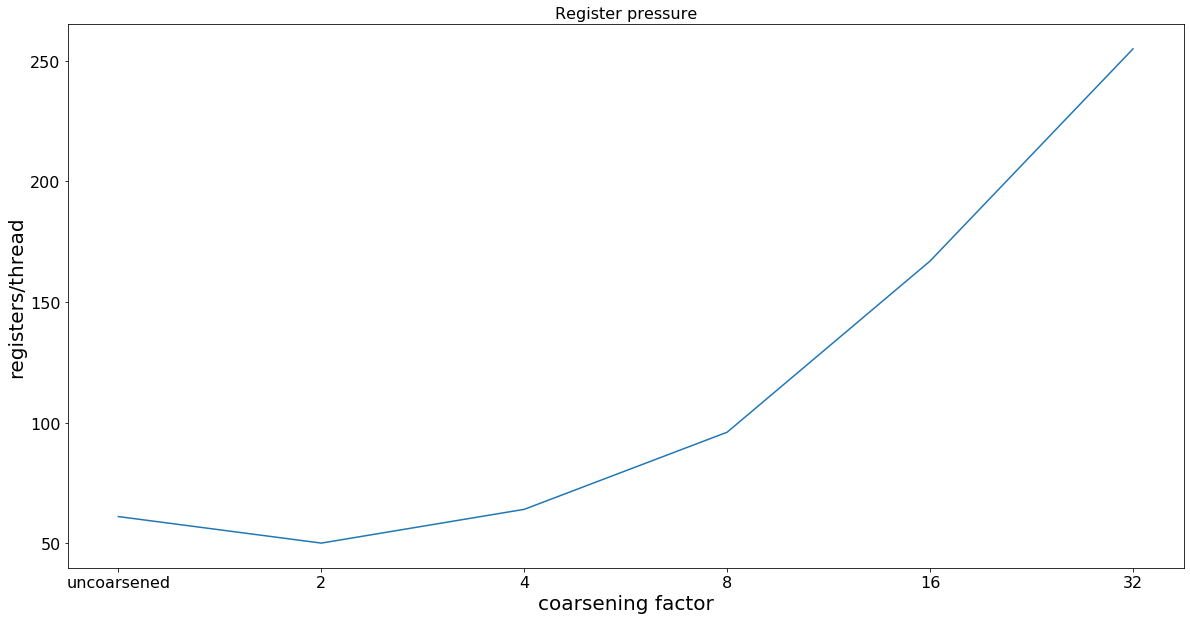
\includegraphics[scale=0.30]{Pictures/plots/poor_improvement/reg pressure.png}
	\caption{\small Register pressures for differently coarsened kernels - Case II}
\end{figure}

Notice that this trend is identical to what we saw in the previous case (fig. 3.8)! This reinforces our previous conclusion that occupancy (and the execution time observed) is not a uni-variate function (of register pressure) but depends on a lot of factors instead.

\begin{table}[ht]
    \centering
    
    \begin{tabular}{ |p{2cm}|p{1.5cm}|p{1.5cm}|p{2cm}|p{2cm}|p{2cm}|p{2cm}|  }
         \hline
         Coarsening factor & Block size & Register pressure & Theoretical Occupancy & Achieved Occupancy & SM Utilization & Execution time (in ms) \\
         \hline
         
         1                  & 992 & 61 & 96.88 & 96.01 & 64.63 & 19.97\\
         2                  & 512 & 50 & 100 & 99.31 & 68.09 & 19.73\\
         4                  & 256 & 64 & 100 & 98.81 & 68.09 & 19.72\\
         8                  & 128 & 96 & 62.5 & 61.42 & 68.02 & 19.74\\
         16                 & 64 & 167 & 31.25 & 30.84 & 66.56 & 20.14\\
         32                 & 32 & 255 & 15.62 & 15.47 & 37.55 & 36.53\\
         \hline
    \end{tabular}
    \caption{\small Comparison of occupancy and execution time variation with coarsening factor - Case II}
    \label{tab:block_size_good_coarsen}
\end{table}

Notice how the occupancy for the uncoarsened kernel is already quite high. While coarsening initially does lead to a very slight increase in the occupancy, both theoretical and achieved, it falls quite rapidly as the coarsening factor increases. Thus, we observe that in cases where the occupancy of the kernel is high, coarsening isn't a very suitable optimization. The reason why this happens is because of the inherent trade-off that coarsening embodies. The reduction in parallelism in exchange for a smaller block size or more coarsened threads is not very beneficial as the occupancy is already quite high, suggesting that the number of concurrently scheduled blocks on the SM is not being a bottleneck. However, further coarsening can, and does as the data suggests, lead to a reduction in the occupancy since the greater resource demand (in terms of register pressure) by each warp causes fewer warps to be active at any given moment, owing to the finite number of registers in each SM. Hence, we can conclude that when the size of the thread block is not being a bottleneck in the occupancy, reducing its size through coarsening does not influence the performance in any non-trivial manner. On the flip side, the increased register pressure introduced by coarsening can easily start to dominate and become a bottleneck in the occupancy calculations.

The results for this set of hyper-parameters are summarized in table 3.2.





% Chapter Template

\chapter{Conclusion} % Main chapter title

\label{Chapter 4} % Change X to a consecutive number; for referencing this chapter elsewhere, use \ref{ChapterX}

\lhead{Chapter 4. \emph{Conclusion}} % Change X to a consecutive number; this is for the header on each page - perhaps a shortened title

%----------------------------------------------------------------------------------------
%	SECTION 1
%---------------------------------------------------------------------------------------

The work done for the Bachelor Thesis Project - I this semester is part of a larger project aimed at developing a scheduling system capable of automatically scheduling multiple kernels on CUDA streams with the appropriate optimizations done in the form of kernel fusion and thread and block coarsening. The decisions regarding scheduling and optimizations done will be taken by the system on the basis of the available system resources.

The work done this semester focused on the first part of the project which included implementing a parameterized pass that can coarsen computational kernels pertaining to CNN pipelines with ease. In addition, we studied the behavior of convolution kernels when coarsened to different extents to understand the trends in performance achieved by these kernel variants under different sets of hyper-parameters.

The upcoming objectives would be to consider multiple pipelines, and while dispatching independent kernels simultaneously, design a heuristic for deciding the individual coarsening parameters for each kernel that would result in efficiently utilizing the hardware resources.


%----------------------------------------------------------------------------------------
%	THESIS CONTENT - APPENDICES
%----------------------------------------------------------------------------------------

\addtocontents{toc}{\vspace{2em}} % Add a gap in the Contents, for aesthetics

\appendix % Cue to tell LaTeX that the following 'chapters' are Appendices

% Include the appendices of the thesis as separate files from the Appendices folder
% Uncomment the lines as you write the Appendices

%\input{Appendices/AppendixA}
%\input{Appendices/AppendixB}
%\input{Appendices/AppendixC}

\addtocontents{toc}{} % Add a gap in the Contents, for aesthetics

\backmatter

%----------------------------------------------------------------------------------------
%	BIBLIOGRAPHY
%----------------------------------------------------------------------------------------
%\nocite{*}
\label{Bibliography}

\begin{thebibliography}{00}
\bibitem{b1} N. Stawinoga and T. Field, ``Predictable Thread Coarsening,'' ACM Transactions on Architecture and Code Optimization, Vol. 15, No. 2, Article 23, June 2018

\bibitem{b1} J. Cheng, M. Grossman, T. McKercher, ``Professional CUDA C Programming``, Wiley, October 2014



\end{thebibliography}

\end{document}